\documentclass[border=10pt]{standalone}
\usepackage{tikz}
\usetikzlibrary{arrows.meta, shadows.blur, backgrounds, calc}

\begin{document}
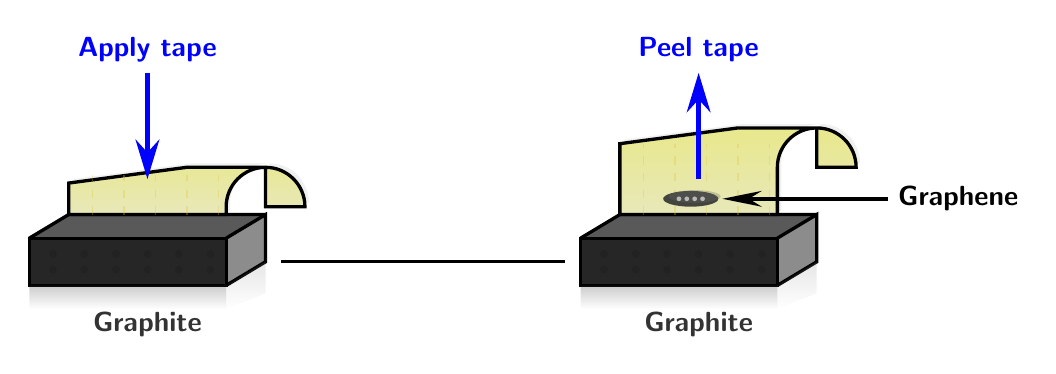
\begin{tikzpicture}[
  font=\sffamily\bfseries,
  line width=1pt
]

% ------------------- Left: Apply Tape ------------------- %
\begin{scope}

  % Graphite block (3D with enhanced shading)
  \fill[black!85] (0,0) rectangle (2.5,0.6);
  \fill[black!45] (2.5,0) -- (3,0.3) -- (3,0.9) -- (2.5,0.6) -- cycle;
  \fill[black!65] (0,0.6) -- (2.5,0.6) -- (3,0.9) -- (0.5,0.9) -- cycle;
  
  % Add subtle texture to graphite
  \foreach \i in {0.3,0.7,1.1,1.5,1.9,2.3} {
    \foreach \j in {0.2,0.4} {
      \fill[black!90, opacity=0.3] (\i,\j) circle (0.05);
    }
  }
  
  % Outlines with slightly thicker lines
  \draw[line width=1.2pt] (0,0) rectangle (2.5,0.6);
  \draw[line width=1.2pt] (2.5,0) -- (3,0.3) -- (3,0.9) -- (2.5,0.6);
  \draw[line width=1.2pt] (0,0.6) -- (0.5,0.9) -- (3,0.9);
  
  % Realistic reflection under the graphite block - front face
  \begin{scope}[transparency group, opacity=0.25]
    \fill[black!80, path fading=south] (0,0) -- (2.5,0) -- (2.5,-0.3) -- (0,-0.3) -- cycle;
  \end{scope}
  
  % Realistic reflection under the graphite block - right face
  \begin{scope}[transparency group, opacity=0.2]
    \fill[black!50, path fading=south] (2.5,0) -- (3,0.3) -- (3,-0.1) -- (2.5,-0.3) -- cycle;
  \end{scope}
  
  % Tape with enhanced shading and 3D effect
  \begin{scope}
    % Shadow underneath tape for 3D effect
    \fill[black!30, opacity=0.2] (0.55,0.95) -- (2.55,0.95) -- (2.55,1.05) 
      arc[start angle=180, end angle=0, radius=0.5]
      -- (3.05,1.05) -- (3.05,1.55) -- (2.05,1.55) -- (0.55,1.35) -- cycle;
  \end{scope}


   % Tape with gradient fill for better 3D appearance
   \fill[top color=yellow!35, bottom color=yellow!20, opacity=0.9] 
     (0.5,0.9) -- (2.5,0.9) -- (2.5,1.0) 
     arc[start angle=180, end angle=0, radius=0.5]
     -- (3.0,1.0) -- (3.0,1.5) -- (2.0,1.5) -- (0.5,1.3) -- cycle;
  
  % Outline of tape
  \draw[line width=1.2pt] 
    (0.5,0.9) -- (2.5,0.9) -- (2.5,1.0) 
    arc[start angle=180, end angle=0, radius=0.5]
    -- (3.0,1.0) -- (3.0,1.5) -- (2.0,1.5) -- (0.5,1.3) -- cycle;
  
  % Add subtle pattern/texture to tape
  \foreach \i in {0.8,1.2,1.6,2.0,2.4} {
    \draw[yellow!50!brown, opacity=0.3, dashed, line width=0.5pt] (\i,0.9) -- (\i,1.4);
  }
  
  % Arrow: Apply tape (downward) - with enhanced styling
  \draw[-{Stealth[length=5mm,width=3mm]}, blue, line width=2pt] (1.5,2.7) -- (1.5,1.35);
  \node[blue, align=center, font=\sffamily\bfseries] at (1.5,3.0) {Apply tape};
  
  % Label with subtle shadow
  \node[font=\sffamily\bfseries, text=black!80] at (1.5,-0.5) {Graphite};
\end{scope}

% ------------------- Right: Peel Tape ------------------- %
\begin{scope}[xshift=7cm]

  % Graphite block (3D with enhanced shading)
  \fill[black!85] (0,0) rectangle (2.5,0.6);
  \fill[black!45] (2.5,0) -- (3,0.3) -- (3,0.9) -- (2.5,0.6) -- cycle;
  \fill[black!65] (0,0.6) -- (2.5,0.6) -- (3,0.9) -- (0.5,0.9) -- cycle;
  
  % Add subtle texture to graphite
  \foreach \i in {0.3,0.7,1.1,1.5,1.9,2.3} {
    \foreach \j in {0.2,0.4} {
      \fill[black!90, opacity=0.3] (\i,\j) circle (0.05);
    }
  }
  
  % Outlines with slightly thicker lines
  \draw[line width=1.2pt] (0,0) rectangle (2.5,0.6);
  \draw[line width=1.2pt] (2.5,0) -- (3,0.3) -- (3,0.9) -- (2.5,0.6);
  \draw[line width=1.2pt] (0,0.6) -- (0.5,0.9) -- (3,0.9);
  
  % Realistic reflection under the graphite block - front face
  \begin{scope}[transparency group, opacity=0.25]
    \fill[black!80, path fading=south] (0,0) -- (2.5,0) -- (2.5,-0.3) -- (0,-0.3) -- cycle;
  \end{scope}
  
  % Realistic reflection under the graphite block - right face
  \begin{scope}[transparency group, opacity=0.2]
    \fill[black!50, path fading=south] (2.5,0) -- (3,0.3) -- (3,-0.1) -- (2.5,-0.3) -- cycle;
  \end{scope}
  
  % Shadow underneath tape for 3D effect
  \fill[black!30, opacity=0.2] (0.55,0.95) -- (2.55,0.95) -- (2.55,1.55) 
    arc[start angle=180, end angle=0, radius=0.5]
    -- (3.05,1.55) -- (3.05,2.05) -- (2.05,2.05) -- (0.55,1.85) -- cycle;
  
  % Tape with gradient fill for better 3D appearance
  \fill[top color=yellow!40, bottom color=yellow!20, opacity=0.9] 
    (0.5,0.9) -- (2.5,0.9) -- (2.5,1.5) 
    arc[start angle=180, end angle=0, radius=0.5]
    -- (3.0,1.5) -- (3.0,2.0) -- (2.0,2.0) -- (0.5,1.8) -- cycle;
  
  % Outline of tape
  \draw[line width=1.2pt] 
    (0.5,0.9) -- (2.5,0.9) -- (2.5,1.5) 
    arc[start angle=180, end angle=0, radius=0.5]
    -- (3.0,1.5) -- (3.0,2.0) -- (2.0,2.0) -- (0.5,1.8) -- cycle;
  
  % Add subtle pattern/texture to tape
  \foreach \i in {0.8,1.2,1.6,2.0,2.4} {
    \draw[yellow!50!brown, opacity=0.3, dashed, line width=0.5pt] (\i,0.9) -- (\i,1.8);
  }
  
  % Graphene flake on tape with shadow/3D effect
  \fill[black!80, opacity=0.9] (1.4,1.1) ellipse (0.35 and 0.1);
  \fill[black!60, opacity=0.3] (1.45,1.13) ellipse (0.33 and 0.08);
  
  % Add hexagonal pattern to graphene flake to represent structure
  \foreach \i in {1.25,1.35,1.45,1.55} {
    \fill[white, opacity=0.6] (\i,1.1) circle (0.03);
  }
  
  % Upward arrow with enhanced styling
  \draw[-{Stealth[length=5mm,width=3mm]}, blue, line width=2pt] (1.5,1.35) -- (1.5,2.7);
  \node[blue, align=center, font=\sffamily\bfseries] at (1.5,3.0) {Peel tape};
  
  % Graphene label with enhanced arrow
  \draw[-{Stealth[length=5mm,width=2mm]}, black, line width=1.5pt](3.9,1.1) -- (1.8,1.1);
  \node[right, font=\sffamily\bfseries, align=left] at (3.9,1.1) {Graphene};
  
  % Label with subtle shadow
  \node[font=\sffamily\bfseries, text=black!80] at (1.5,-0.5) {Graphite};
\end{scope}

% Add a decorative connection between the two diagrams
\draw[line width=1pt, opacity=1, black] (3.2,0.3) -- (6.8,0.3);

\end{tikzpicture}
\end{document}
